\documentclass[aspectratio=169]{beamer}
% SGSSS Beamer Preamble — shared across all lectures
% Brand colours from SGSSS logo

\usetheme{metropolis}

% --- Colour definitions ---
\definecolor{sgsssMagenta}{HTML}{A3217A}
\definecolor{sgsssGreen}{HTML}{2D6A3F}
\definecolor{sgsssBlack}{HTML}{1D1D1B}
\definecolor{sgsssWhite}{HTML}{FFFFFF}
\definecolor{sgsssLightGrey}{HTML}{F5F5F5}

% --- Metropolis colour overrides ---
\setbeamercolor{palette primary}{bg=sgsssMagenta, fg=sgsssWhite}
\setbeamercolor{title separator}{fg=sgsssGreen}
\setbeamercolor{progress bar}{fg=sgsssGreen, bg=sgsssLightGrey}
\setbeamercolor{frametitle}{bg=sgsssMagenta, fg=sgsssWhite}
\setbeamercolor{alerted text}{fg=sgsssMagenta}
\setbeamercolor{example text}{fg=sgsssGreen}
\setbeamercolor{block title}{bg=sgsssMagenta, fg=sgsssWhite}
\setbeamercolor{block body}{bg=sgsssLightGrey, fg=sgsssBlack}
\setbeamercolor{block title example}{bg=sgsssGreen, fg=sgsssWhite}
\setbeamercolor{block body example}{bg=sgsssLightGrey, fg=sgsssBlack}
\setbeamercolor{block title alerted}{bg=sgsssMagenta, fg=sgsssWhite}
\setbeamercolor{block body alerted}{bg=sgsssLightGrey, fg=sgsssBlack}
\setbeamercolor{normal text}{fg=sgsssBlack}

% --- Fonts ---
\usepackage[T1]{fontenc}
\usepackage[sfdefault]{FiraSans}
\usepackage{FiraMono}
\setbeamerfont{frametitle}{size=\large}

% --- Packages ---
\usepackage{graphicx}
\usepackage{bookmark}
\hypersetup{
    bookmarks=true,
    bookmarksopen=true,
    bookmarksdepth=2,
    pdfpagemode=UseOutlines,
}
% --- PDF bookmarks for each frame title ---
\makeatletter
\apptocmd{\beamer@@frametitle}{%
  \only<1>{\bookmark[page=\the\c@page,level=1]{#1}}%
}{}{}
\makeatother
\usepackage{array}
\usepackage{booktabs}
\usepackage{minted}
\usepackage{fontawesome5}

% --- TikZ ---
\usepackage{tikz}
\usetikzlibrary{arrows.meta, positioning, shapes.geometric, trees, calc, decorations.pathmorphing, decorations.pathreplacing, fit, backgrounds}

% Reusable TikZ styles
\tikzset{
    server node/.style={rectangle, draw=sgsssGreen, fill=sgsssGreen!10, thick, minimum width=2.5cm, minimum height=1.2cm, align=center, font=\small},
    client node/.style={rectangle, draw=sgsssMagenta, fill=sgsssMagenta!10, thick, minimum width=2.5cm, minimum height=1.2cm, align=center, font=\small},
    api node/.style={rectangle, draw=sgsssGreen, fill=sgsssGreen!15, thick, rounded corners, minimum width=2.5cm, minimum height=1.2cm, align=center, font=\small},
    data node/.style={rectangle, draw=sgsssBlack, fill=sgsssLightGrey, thick, minimum width=2cm, minimum height=1cm, align=center, font=\small},
    arrow style/.style={-{Stealth[length=3mm]}, thick, sgsssBlack},
    html tag/.style={rectangle, draw=sgsssMagenta, fill=sgsssMagenta!8, rounded corners=2pt, font=\ttfamily\small, inner sep=4pt},
    json key/.style={rectangle, draw=sgsssGreen, fill=sgsssGreen!8, rounded corners=2pt, font=\ttfamily\small, inner sep=4pt},
}

% --- Minted configuration ---
\setminted{
    fontsize=\footnotesize,
    frame=leftline,
    framesep=2mm,
    baselinestretch=1.1,
    bgcolor=sgsssLightGrey,
    breaklines,
    linenos=false,
}
\setminted[python]{style=friendly}
\setminted[r]{style=friendly}

% --- Convenience commands ---
\newcommand{\pythoncode}[1]{\mintinline{python}{#1}}
\newcommand{\rcode}[1]{\mintinline{r}{#1}}
\newcommand{\httpstatus}[2]{\texttt{#1} \textit{#2}}

% --- Footer (page numbers only; logo on title slide only) ---
\setbeamertemplate{frame footer}{%
    \insertframenumber/\inserttotalframenumber%
}

% --- Metadata ---
\author{Dr Diarmuid McDonnell}
\institute{Braw Data Ltd \and Gradel Institute of Charity, University of Oxford}
\date{27 March 2026}


\title{Text Analysis for Social Scientists}
\subtitle{SGSSS Training Course}

\begin{document}

% -------------------------------------------------------
% Slide 1: Title
% -------------------------------------------------------
{
\setbeamertemplate{frame footer}{}
\begin{frame}[plain]
    \begin{center}
        
\includegraphics[height=2.5cm]{../img/SGSSS_Stacked.png}\\[0.8cm]
        {\Large\bfseries\color{sgsssMagenta} Text Analysis for Social Scientists}\\[0.2cm]
        {\large SGSSS Training Course}\\[0.6cm]
        {\normalsize Dr Diarmuid McDonnell}\\[0.1cm]
        {\small Braw Data Ltd \(\cdot\) Gradel Institute of Charity, University of Oxford}\\[0.3cm]
        {\small 27 March 2026}
    \end{center}
\end{frame}
}

% -------------------------------------------------------
% Slide 2: About the instructor
% -------------------------------------------------------
\begin{frame}{About the Instructor}
    \textbf{Dr Diarmuid McDonnell}
    \begin{itemize}
        \item Director, \textbf{Braw Data Ltd}
        \item Visiting Fellow, \textbf{Gradel Institute of Charity}, University of Oxford
        \item Research: computational social science, civil society, philanthropy
        \item Background in quantitative social science and data science
    \end{itemize}
    \vspace{0.3cm}
    {\small \faIcon{globe} \url{https://www.brawdata.co.uk}}\\
    {\small \faIcon{university} \url{https://www.gradelinstituteofcharity.co.uk/diarmuid-mcdonnell}}
\end{frame}

% -------------------------------------------------------
% Slide 3: Course outline
% -------------------------------------------------------
\begin{frame}{Course Outline}
    \footnotesize
    \begin{tabular}{@{}lll@{}}
        \toprule
        \textbf{Time} & \textbf{Session} & \textbf{Format} \\
        \midrule
        10:00--10:30 & Welcome \& Text as Data & Lecture \\
        10:30--11:00 & \alert{Practical 1: Preprocessing Text} & Colab notebook \\
        11:00--11:15 & Break & \\
        11:15--11:30 & Exploring Text & Lecture \\
        11:30--12:15 & \alert{Practical 2: Descriptive Text Analysis} & Colab notebook \\
        12:15--13:00 & Lunch & \\
        13:00--13:30 & Topic Modelling & Lecture \\
        13:30--14:45 & \alert{Practical 3: Topic Modelling} & Colab notebook \\
        14:45--15:00 & Break & \\
        15:00--15:15 & LLMs for Text Analysis & Lecture \\
        15:15--15:50 & \alert{Practical 4: LLM-Assisted Text Analysis} & Colab notebook \\
        15:50--16:00 & Wrap-up \& Q\&A & \\
        \bottomrule
    \end{tabular}
\end{frame}

% -------------------------------------------------------
% Slide 4: Getting set up
% -------------------------------------------------------
\begin{frame}{Getting Set Up}
    \begin{block}{What you need}
        \begin{itemize}
            \item A \textbf{Google account} (for Google Colab)
            \item A web browser (Chrome recommended)
        \end{itemize}
    \end{block}

    \begin{block}{How to access the notebooks}
        \begin{enumerate}
            \item Go to the course \textbf{README} (link shared on Teams/email)
            \item Click the \textbf{Open in Colab} badge for your chosen language
            \item Materials available in \textbf{Python} and \textbf{R}
            \item Sign in with your Google account --- you're ready to go!
        \end{enumerate}
    \end{block}

    \vspace{0.2cm}
    {\small \faIcon{info-circle} No software installation required --- everything runs in the browser.}
\end{frame}

% -------------------------------------------------------
% Slide 5: What is quantitative text analysis?
% -------------------------------------------------------
\begin{frame}{What Is Quantitative Text Analysis?}
    \small
    \begin{alertblock}{Key idea}
        Treating \textbf{text as data} --- applying systematic, computational methods to extract meaning from large collections of text.
    \end{alertblock}

    \textbf{Social science applications:}
    \begin{itemize}\setlength\itemsep{0pt}
        \item Analysing \textbf{political speeches} and party manifestos
        \item Tracking \textbf{media coverage} across outlets and over time
        \item Classifying \textbf{policy documents} and legislation
        \item Studying \textbf{online discourse} on social media platforms
    \end{itemize}

    \begin{exampleblock}{Key references}
        \footnotesize
        Grimmer \& Stewart (2013) \(\cdot\)
        Gentzkow, Kelly \& Taddy (2019) \(\cdot\)
        Grimmer, Roberts \& Stewart (2022) \textit{Text as Data}
    \end{exampleblock}
\end{frame}

% -------------------------------------------------------
% Slide 6: The text analysis pipeline
% -------------------------------------------------------
\begin{frame}{The Text Analysis Pipeline}
    \begin{center}
    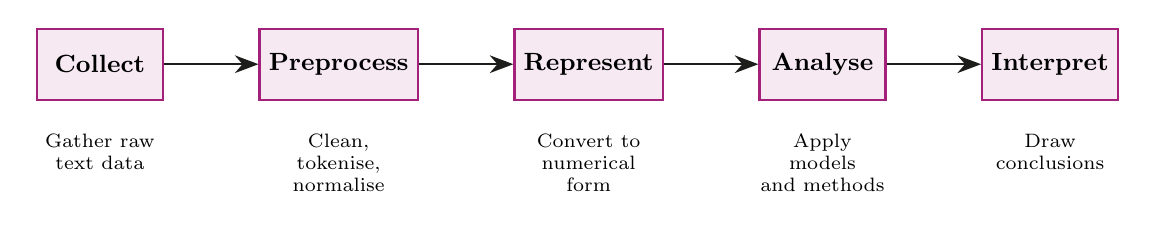
\begin{tikzpicture}[node distance=1.2cm]
        % Define pipeline style
        \tikzset{
            pipeline node/.style={rectangle, draw=sgsssMagenta, fill=sgsssMagenta!10, thick,
                minimum width=1.6cm, minimum height=0.9cm, align=center, font=\small\bfseries},
            desc label/.style={font=\scriptsize, align=center, text width=1.6cm},
        }

        % Nodes
        \node[pipeline node] (collect) {Collect};
        \node[pipeline node, right=of collect] (preprocess) {Preprocess};
        \node[pipeline node, right=of preprocess] (represent) {Represent};
        \node[pipeline node, right=of represent] (analyse) {Analyse};
        \node[pipeline node, right=of analyse] (interpret) {Interpret};

        % Arrows
        \draw[arrow style] (collect) -- (preprocess);
        \draw[arrow style] (preprocess) -- (represent);
        \draw[arrow style] (represent) -- (analyse);
        \draw[arrow style] (analyse) -- (interpret);

        % Descriptions below
        \node[desc label, below=0.3cm of collect] {Gather raw\\text data};
        \node[desc label, below=0.3cm of preprocess] {Clean, tokenise,\\normalise};
        \node[desc label, below=0.3cm of represent] {Convert to\\numerical form};
        \node[desc label, below=0.3cm of analyse] {Apply models\\and methods};
        \node[desc label, below=0.3cm of interpret] {Draw\\conclusions};
    \end{tikzpicture}
    \end{center}

    \vspace{0.3cm}
    {\small Today we will work through each of these stages using real-world text data.}
\end{frame}

% -------------------------------------------------------
% Slide 7: Key concepts
% -------------------------------------------------------
\begin{frame}{Key Concepts}
    \begin{description}[\textbf{Vocabulary}]
        \item[\textbf{Corpus}] A collection of documents (e.g., all speeches by a politician)
        \item[\textbf{Document}] A single unit of text (e.g., one speech, one tweet)
        \item[\textbf{Token}] An individual occurrence of a word or term
        \item[\textbf{Type}] A unique word form in the vocabulary
        \item[\textbf{Vocabulary}] The set of all unique types in a corpus
    \end{description}

    \vspace{0.4cm}
    \begin{exampleblock}{Example}
        \textit{``The cat sat on the mat''}\\[0.2cm]
        \textbf{Tokens:} The, cat, sat, on, the, mat \(\rightarrow\) \textbf{6 tokens}\\
        \textbf{Types:} the, cat, sat, on, mat \(\rightarrow\) \textbf{5 types}
    \end{exampleblock}
\end{frame}

% -------------------------------------------------------
% Slide 8: Structured vs unstructured text
% -------------------------------------------------------
\begin{frame}{Structured vs Unstructured Text}
    \begin{columns}[T]
        \begin{column}{0.47\textwidth}
            \textbf{\color{sgsssMagenta} Unstructured Text}
            \begin{itemize}
                \item Raw text documents
                \item OCR output from scanned pages
                \item Web scrapes (HTML, forums)
                \item Free-text survey responses
                \item Social media posts
            \end{itemize}
            \vspace{0.3cm}
            {\small Requires significant preprocessing before analysis.}
        \end{column}
        \begin{column}{0.47\textwidth}
            \textbf{\color{sgsssGreen} Structured Text}
            \begin{itemize}
                \item CSV with a text column
                \item Labelled corpus (e.g., sentiment)
                \item Annotated datasets
                \item Metadata-rich collections
                \item Pre-processed term--document matrices
            \end{itemize}
            \vspace{0.3cm}
            {\small Ready (or nearly ready) for quantitative analysis.}
        \end{column}
    \end{columns}
\end{frame}

% -------------------------------------------------------
% Slide 9: Ethics of computational text analysis
% -------------------------------------------------------
\begin{frame}{Ethics of Computational Text Analysis}
    \begin{itemize}
        \item \faIcon{user-shield} \textbf{Consent and privacy} --- social media users may not expect their posts to be analysed; consider anonymisation and platform ToS
        \item \faIcon{balance-scale} \textbf{Bias in algorithms} --- text models can encode and amplify societal biases present in training data
        \item \faIcon{database} \textbf{Representativeness of corpora} --- whose voices are included and whose are missing? Consider selection effects
        \item \faIcon{microscope} \textbf{Transparency and reproducibility} --- document preprocessing choices, share code and data where possible
    \end{itemize}

    \vspace{0.3cm}
    \begin{exampleblock}{Guiding principle}
        Computational methods amplify the researcher's reach --- ethical scrutiny should be amplified too.
    \end{exampleblock}
\end{frame}

% -------------------------------------------------------
% Slide 10: Next up
% -------------------------------------------------------
\begin{frame}{Next Up}
    \begin{center}
        {\Large \alert{Practical 1: Preprocessing Text}}\\[0.5cm]
        \begin{itemize}
            \item Tokenise and clean real-world text data
            \item Remove stopwords, punctuation, and noise
            \item Stem and lemmatise tokens
            \item Build a document--term matrix
        \end{itemize}
        \vspace{0.5cm}
        {\normalsize Open the \textbf{Practical 1} notebook in Google Colab\\(Python or R --- your choice!)}
    \end{center}
\end{frame}

\end{document}
